\chapter{Network architecture}
\label{chap:network_architecture}

  This chapter is meant to provide the necessary background needed to
  understand the next chapters. It does not give a complete overview of
  the network architecture, but just enough information to serve as a
  guide for the reader. It is also focused on \gls{gsm} and \gls{gprs}
  only. The information is extracted from the \gls{3gpp} specifications
  which are freely available for anyone wanting to find out more about
  this topic~\cite{3gpp_specifications_????}.

  The mobile network is called the \gls{plmn} infrastructure and is
  represented on~\fref{fig:network_architecture}. It is composed of the
  \gls{cn}, the \gls{an}, and the \gls{ms}. The first section focuses on
  the \gls{cn}, the second section looks at the \gls{an}, and the third
  section is dedicated to the \gls{ms}. The Um interface, connecting the
  \gls{an} and the \gls{ms}, will be introduced
  in~\Cref{chap:protocol_stack_implementation} along with its
  implementation in \proj{OsmocomBB}~\cite{etsi_gsm_2001,3gpp_ts_2015}.

  \begin{figure}[h]
    \centering
    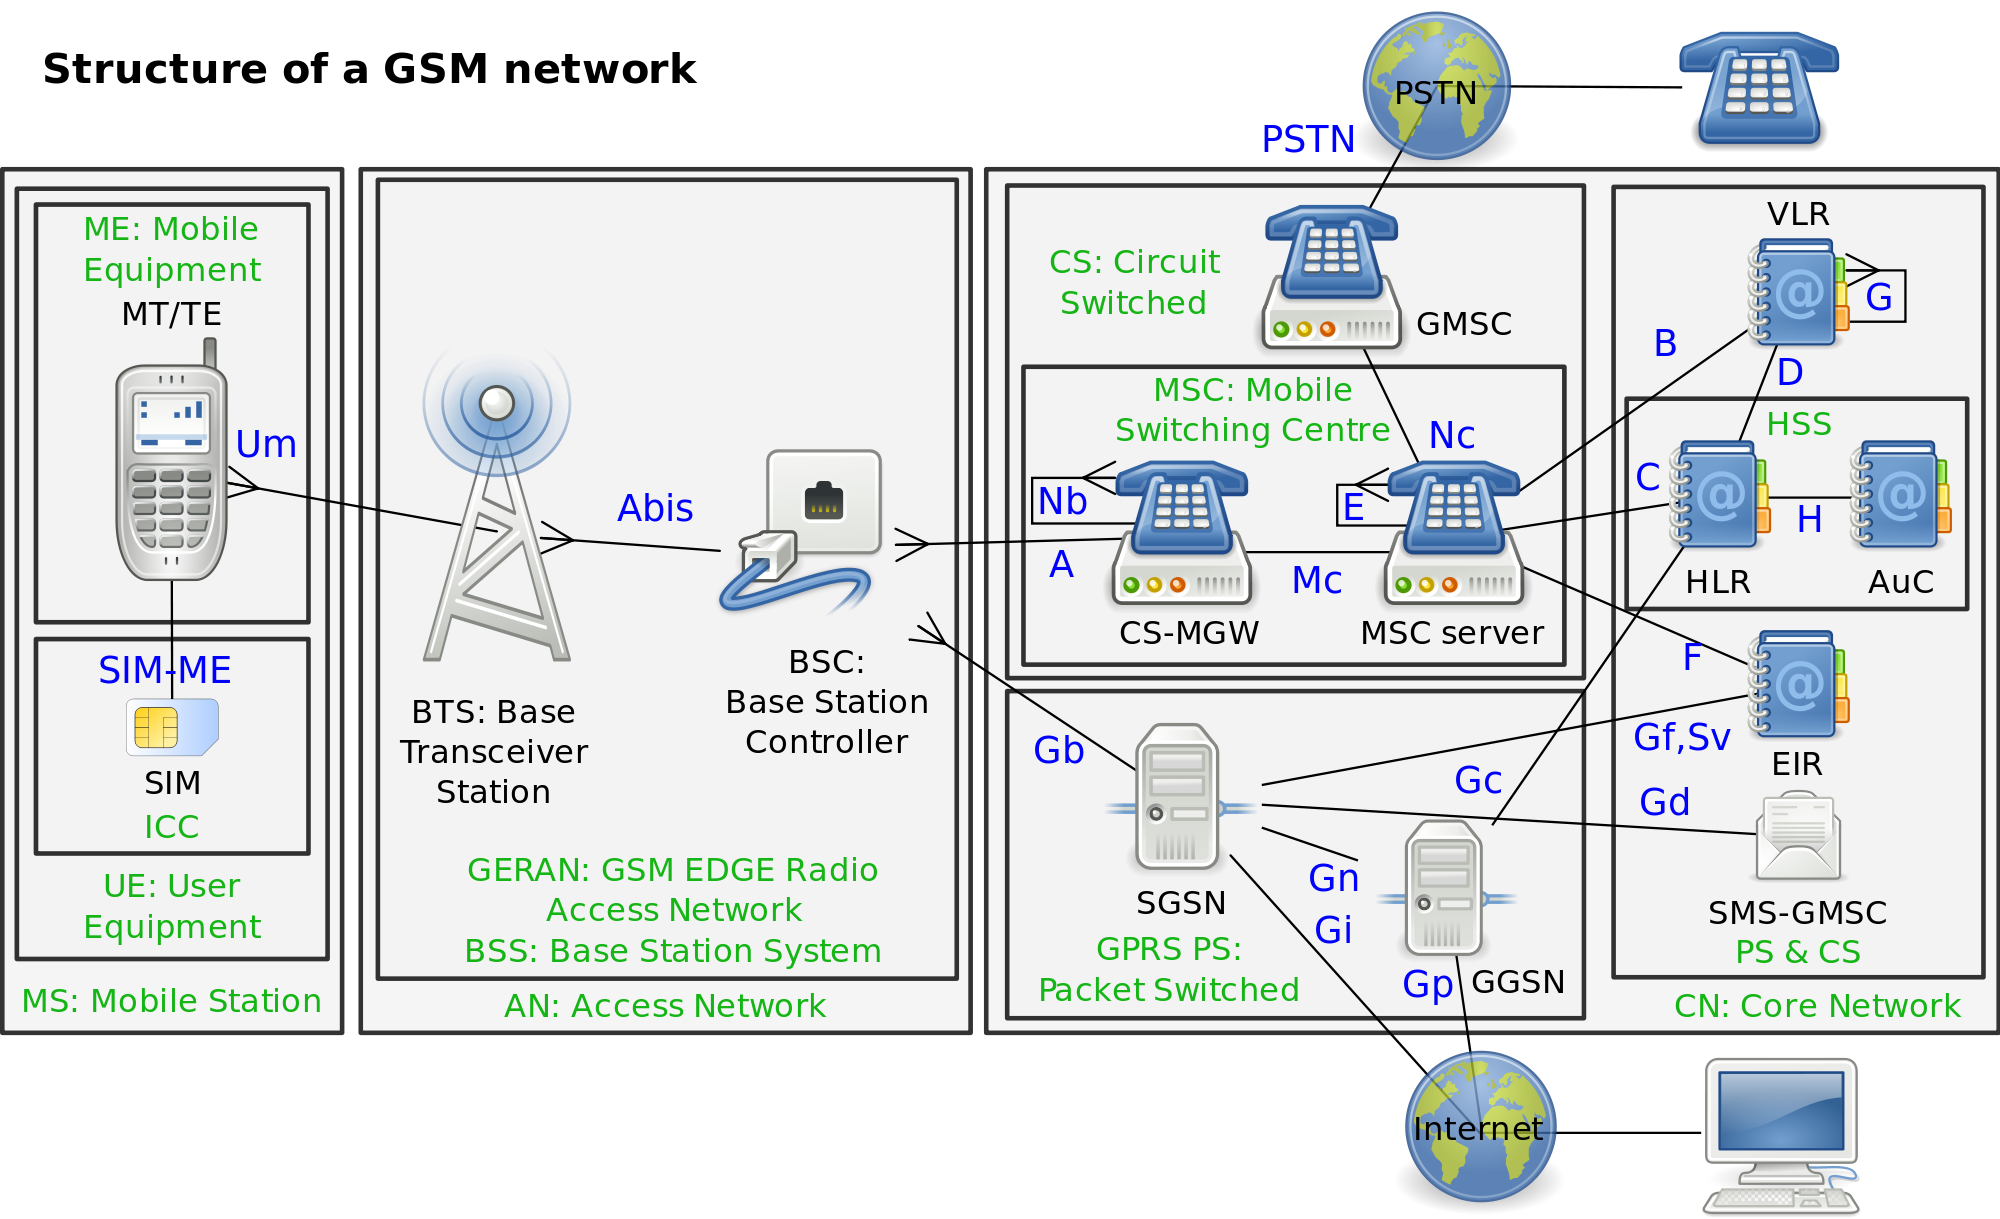
\includegraphics[width=\textwidth]{network_architecture}
    \caption{Key elements of the structure of a GSM
            network~\cite{wikimedia_commons_key_2009}}
    \label{fig:network_architecture}
  \end{figure}

  \section{Core Network entities}

    The \gls{cn} is shown on the right of
    \fref{fig:network_architecture}. It is connected to the \gls{an}, to
    the \gls{pstn} or to the \gls{isdn}, and to the Internet. It is also
    separated between the \gls{cs} domain and the \gls{ps} domain. These
    two domains are overlapping since they contain some common entities,
    but they differ by the way they support user traffic. Basically, the
    entities specific to the \gls{ps} domain are the \gls{gprs} specific
    entities. This section reviews all the relevant \gls{cn} entities in
    turn, and then shortly describes the signaling system used between
    them~\cite{3gpp_ts_2015}.

    \subsection{Home Subscriber Server}

      The \gls{hss} is the entity containing the subscription-related
      information to support the network entities actually handling
      calls or sessions. It is common to the \gls{cs} and \gls{ps}
      domains and contains two different entities: the \gls{hlr} and the
      \gls{auc}~\cite{3gpp_ts_2015}.

      The \gls{hlr} is a database providing a known, fixed location to
      dispense information about an inherently mobile subscriber. It
      stores subscriber information, like the \gls{imsi} and the
      \gls{msisdn}. It also stores location information allowing
      incoming calls to be routed. The \gls{auc} is associated with an
      \gls{hlr} and stores the authentication key Ki for each mobile
      subscriber registered with the associated \gls{hlr}. This key is a
      shared secret between the \gls{auc} and the \gls{sim} and should
      not leave these two entities. It is used with the A3 and A8
      algorithms to generate security data needed for authentication and
      ciphering for each mobile subscriber, for example the session key.
      The \gls{hlr} requests this data from the \gls{auc}, stores it and
      delivers it to the \gls{vlr} and
      \gls{sgsn}~\cite{etsi_gsm_1992,etsi_gsm_2001,3gpp_ts_2015}.

      The \gls{imsi} is a unique number identifying a subscriber on the
      \gls{plmn} and its structure is shown on
      \fref{fig:structure_of_imsi}. It is composed of the \gls{mcc}, the
      \gls{mnc}, and the \gls{msin}. The \gls{mcc} identifies the
      country of origin of the subscriber, the \gls{mnc} identifies the
      home \gls{plmn} of the subscriber within this country, and the
      \gls{msin} identifies the subscriber within this \gls{plmn}. The
      \gls{msisdn} is the phone number of the
      subscriber~\cite{3gpp_ts_2003}.

      \begin{figure}[h]
        \centering
        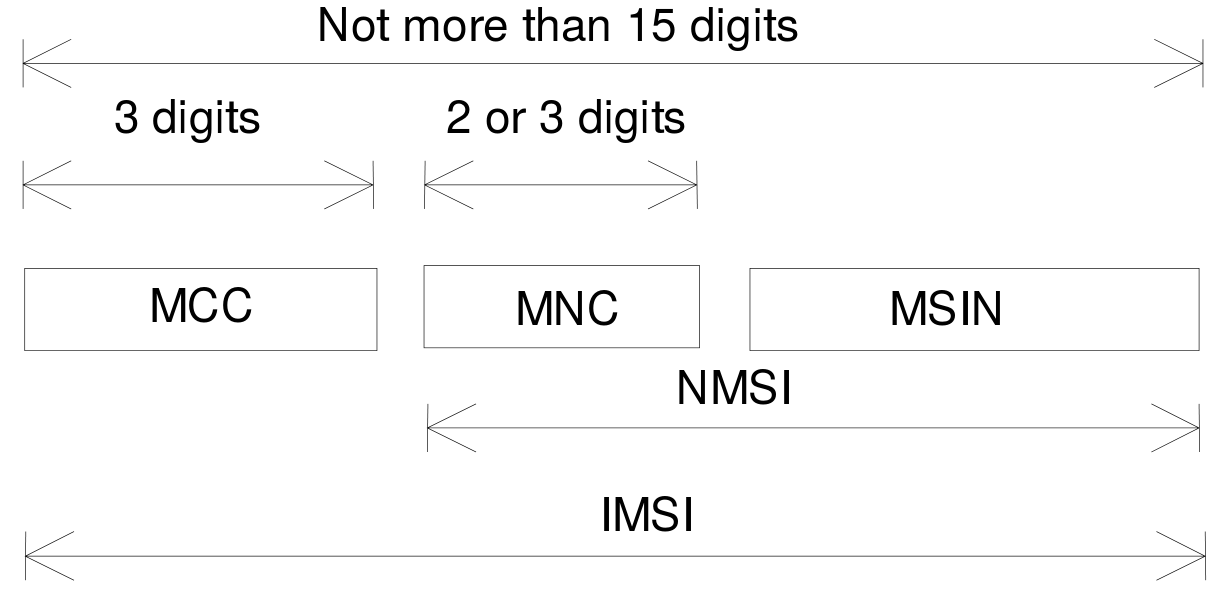
\includegraphics[width=0.7\textwidth]{structure_of_imsi}
        \caption{Structure of an IMSI~\cite{3gpp_ts_2003}}
        \label{fig:structure_of_imsi}
      \end{figure}

    \subsection{Visitor Location Register}

      The \gls{vlr} stores information needed to manage the mobile
      nature of subscribers, when they are located in the \gls{vlr}
      area. It stores identity information, like the \gls{tmsi}, or
      location information, like the \gls{lai} in which the mobile has
      been registered. The \gls{vlr} retrieves information from the
      \gls{hlr} and provides a local storage which is needed to handle
      calls to and from subscribers in the location areas related to the
      \gls{vlr}. The \gls{vlr} is common to the \gls{cs} and \gls{ps}
      domains.

      The \gls{vlr} area is the part of the network controlled by a
      \gls{vlr}. It may consist of one or several \gls{msc} areas. The
      \gls{tmsi} is a temporary number identifying the subscriber
      inside a \gls{vlr} area or inside an \gls{sgsn} area. The
      \gls{la} is defined as an area in which an \gls{ms} may move
      freely without updating the \gls{vlr}. An \gls{lai} is a number
      identifying a location area, and is composed of the \gls{mcc},
      the \gls{mnc}, and the \gls{lac}. This is shown on
      \fref{fig:structure_of_lai}. The \gls{lac} is a number
      identifying a location area within a \gls{plmn}
      ~\cite{etsi_gsm_1992-1,etsi_gsm_2001,3gpp_ts_2003,3gpp_ts_2015}.

      \begin{figure}[h]
        \centering
        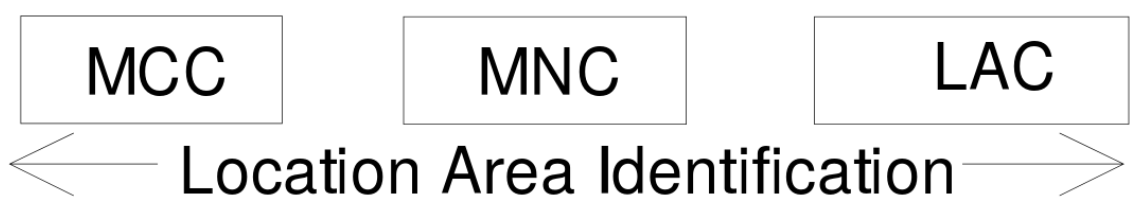
\includegraphics[width=0.5\textwidth]{structure_of_lai}
        \caption{Structure of an \gls{lai}~\cite{3gpp_ts_2003}}
        \label{fig:structure_of_lai}
      \end{figure}

      \iffalse
      GSM 03.08
      0104 def and 0302 full def
      0301. 0303 for tmsi structure
      0308
      \fi

    \subsection{Mobile-services Switching Centre}
    \label{sssection:msc}

      The \gls{msc} constitutes the interface between the radio system
      and the fixed networks. It performs all necessary functions in
      order to handle the circuit switched services to and from the
      \gls{ms}. The \gls{msc} area is the part of the network covered by
      an \gls{msc}. It may consist of one or several location areas, or
      of one or several \gls{bsc} areas.

      The \gls{gmsc} is a specialized \gls{msc}. If a network delivering
      a call to the \gls{plmn} can not interrogate the relevant
      \gls{hlr}, the call is routed to a \gls{gmsc}. This \gls{gmsc}
      will interrogate the appropriate \gls{hlr} and then route the call
      to the \gls{msc} where the \gls{ms} is located. Another
      specialized \gls{msc} is the \gls{sms-gmsc}, which allows
      \gls{sms} messages to be delivered to the \gls{ms}. While the
      \gls{gmsc} is part of the \gls{cs}, the \gls{sms-gmsc} is a common
      entity of the \gls{cs} and \gls{ps} domains~\cite{3gpp_ts_2015}. 

    \subsection{GPRS Support Nodes}

      There are two types of \gls{gsn}: the \gls{ggsn}, and the
      \gls{sgsn}. They constitute the interface between the radio
      system and the fixed networks for packet switched services.
      Together, they perform all necessary functions in order to
      handle the packet transmission to and from the \gls{ms}. The
      \gls{sgsn} area is the part of the network served by an
      \gls{sgsn}. It may consist of one or several routing areas, or
      of one or several \gls{bsc} areas. The \gls{ra} is defined as an
      area in which an \gls{ms} may move freely without updating the
      \gls{sgsn}.

      The \gls{sgsn} has a location register function which stores two
      types of subscriber data needed to handle originating and
      terminating packet data transfer: subscription information,
      including temporary identities, and location information. The
      location register function in the \gls{ggsn} stores subscriber
      data received from the \gls{hlr} and the \gls{sgsn}. It stores
      subscription information, and the address of the \gls{sgsn}
      related to the subscriber~\cite{3gpp_ts_2015}.

    \subsection{MAP protocol of the SS7} 
    \label{sec:ss7}
      
      The \gls{ss7} is used to transfer information between entities of
      the \gls{plmn}, and between \glspl{plmn} and other telephony
      networks. The application level of the \gls{ss7} contains the
      \gls{map} protocol. The \gls{map} is specific to mobile networks,
      and defines various services used to transfer information between
      the entities of the \gls{plmn} defined earlier in this section.
      Three of these services are important for this thesis, and they
      are introduced in this section~\cite{3gpp_ts_2015-2}.

      \subsubsection{MAP-SEND-ROUTING-INFO-FOR-SM}
      \label{sec:sriforsm}

        The MAP-SEND-ROUTING-INFO-FOR-SM service is \textquote{used
        between the gateway MSC and the HLR to retrieve the routing
      information needed for routing the short message to the servicing
    MSC}. This service allows, using a phone number (\gls{msisdn}), to
    request the \gls{imsi} of the related subscriber, as well as the
    number of the \gls{msc} which is serving it. The use of this service
    is illustrated
    on~\fref{fig:map_srifs}~\cite[p.~232]{3gpp_ts_2015-2}.
        
        \begin{enumerate}[topsep=-1em,parsep=0em,itemsep=0em]

          \item The Service Center serving the sending \gls{ms} sends
            the \gls{sms} message to the related \gls{gmsc}.         

          \item This \gls{gmsc} sends a MAP-SEND-ROUTING-INFO-FOR-SM
            request containing the receiving phone number to the
            \gls{hlr} related to that subscriber.

          \item This \gls{hlr} answers with the \gls{imsi} of the
            receiving subscriber, as well as the number of the \gls{msc}
            serving it.

          \item The \gls{gmsc} serving the sender transmits the
            \gls{sms} message to the \gls{msc} serving the receiver.
        
        \end{enumerate}
        
        \begin{figure}[h]
          \centering
          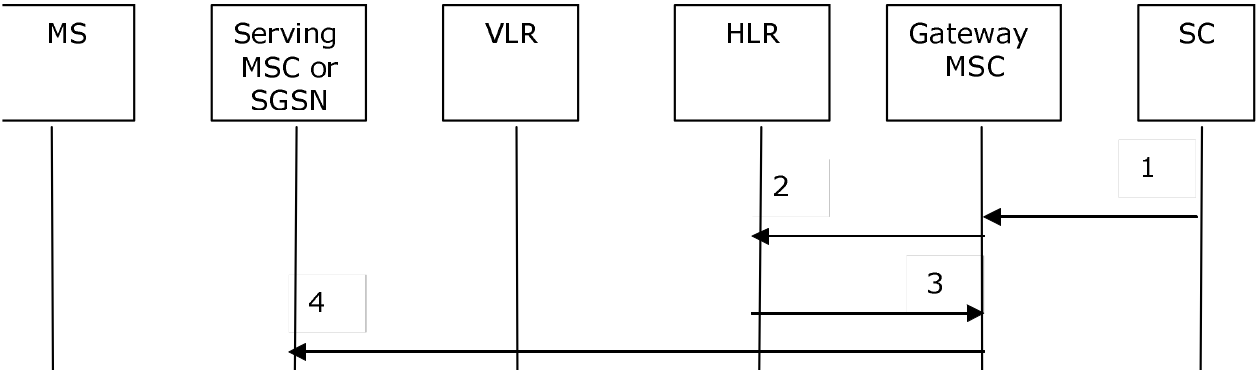
\includegraphics[width=\textwidth]{map_srifs}
          \caption{Beginning of the mobile terminated SMS
          procedure~\cite[p.~792]{3gpp_ts_2015-2}}
          \label{fig:map_srifs}
        \end{figure}

      \subsubsection{MAP-PROVIDE-SUBSCRIBER-Info}
      \label{sec:psi}
          
        The MAP-PROVIDE-SUBSCRIBER-Info service is \textquote{used to
        request information (e.g. subscriber state and location) from
      the VLR or the SGSN at any time}. This service allows, using the
      \gls{imsi} of the subscriber, to request the \gls{cgi} related to
      the phone. An example of this service usage is illustrated
      on~\fref{fig:map_psi}~\cite[p.~181]{3gpp_ts_2015-2}.

        \begin{enumerate}[topsep=-1em,parsep=0em,itemsep=0em]

          \item To establish a call from one \gls{plmn} to another, the
            \gls{msc} of the first network, the VMSC, needs to contact
            the \gls{gmsc} of the second network.

          \item This \gls{gmsc} will contact the \gls{hlr} to request
            the needed routing information.

          \item The \gls{hlr} will then send a
            MAP-PROVIDE-SUBSCRIBER-Info request containing the
            \gls{imsi} of the receiving subscriber.

          \item The \gls{vlr} will answer with the necessary routing
            information, for example the \gls{cgi} of the cell to which
            the receiving subscriber is camping.

        \end{enumerate}

        \begin{figure}[h]
          \centering
          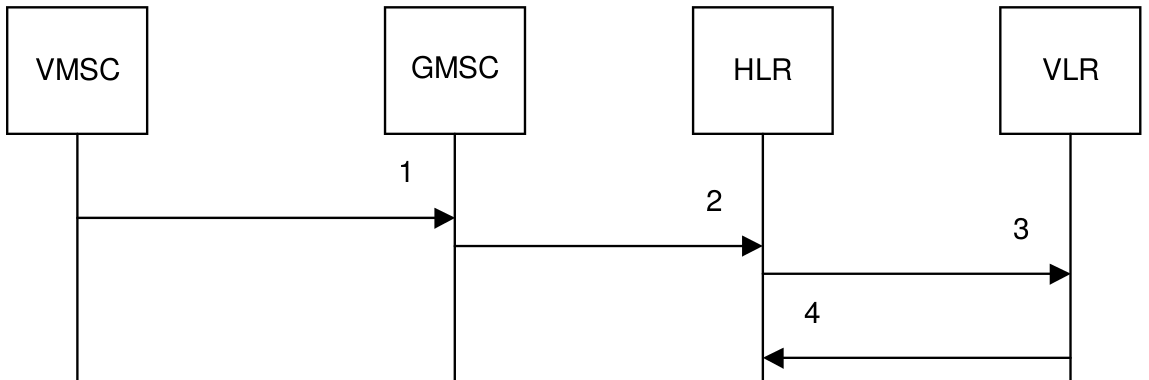
\includegraphics[width=\textwidth]{map_psi}
          \caption{Beginning of the message flow for retrieval of
            routing information~\cite[p.~639]{3gpp_ts_2015-2}}
          \label{fig:map_psi}
        \end{figure}

      \subsubsection{MAP\_SEND\_IDENTIFICATION}
      \label{sec:si}

       The MAP\_SEND\_IDENTIFICATION service \textquote{is used
       between a VLR and a previous VLR to retrieve IMSI and
     authentication data for a subscriber registering afresh in that
   VLR}. This service allows, using the \gls{tmsi} of the phone, to
   request up to five authentication sets, as long as they are
   available. The authentication sets contain information used to
   authenticate the subscriber and to encrypt its communications on the
   Um interface. An example of this service usage is illustrated
   on~\fref{fig:map_si}~\cite[p.~118]{3gpp_ts_2015-2}.

        \begin{enumerate}[topsep=-1em,parsep=0em,itemsep=0em]

          \item When an \gls{ms} wants to send its location to the
            network, it sends a Location Update request message.         

          \item The related \gls{vlr} will then send a
            MAP\_SEND\_IDENTIFICATION request containing the \gls{tmsi}
            of the subscriber to the Previous \gls{vlr}.

          \item This Previous \gls{vlr} will answer to the new \gls{vlr}
            with a response message containing the \gls{imsi} of the
            subscriber, as well as the related authentication sets.

        \end{enumerate}

        \begin{figure}[h]
          \centering
          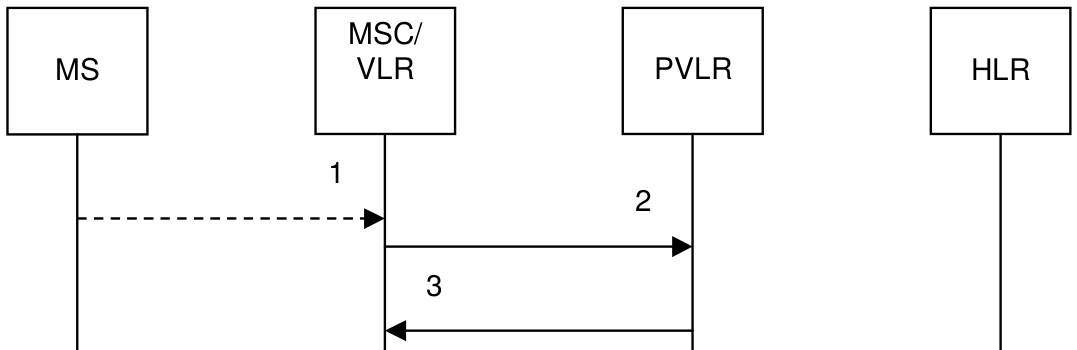
\includegraphics[width=\textwidth]{map_si}
          \caption{Beginning of the message flow for location updating
          to a new VLR area, when the IMSI can be retrieved from the
          previous VLR~\cite[p.~479]{3gpp_ts_2015-2}}
          \label{fig:map_si}
        \end{figure}
      
  \section{Access Network entities}

    After having introduced the \gls{cn} and its entities, this section
    focuses on the \gls{geran}, also called the \gls{bss}, which is
    shown in the middle of \fref{fig:network_architecture}. It is the
    system of base station equipments which is viewed by the \gls{msc}
    as being the entity responsible for communicating with \glspl{ms} in
    a certain area. A \gls{bss} is subdivided into a control function
    carried out by the \gls{bsc} and a radio transmitting function
    carried out by the \gls{bts} with its transceivers, TRX. In order to
    keep the \gls{bts} as simple as possible, it contains only those
    functions which have to reside close to the radio
    interface~\cite{etsi_gsm_2001,3gpp_ts_2002,3gpp_ts_2015}.

    \subsection{Base Station Controller}

      A \gls{bsc} is a network component in the \gls{plmn} with the
      function to control one or more \glspl{bts}. The \gls{bsc} area
      is an area of radio coverage consisting of one or more cells
      controlled by one \gls{bsc}, which is responsible for most of
      the functions of the
      \gls{bss}~\cite{etsi_gsm_2001,3gpp_ts_2002,3gpp_ts_2015}.
 
    \subsection{Base Transceiver Station}
    \label{sec:cgi}

      A \gls{bts} is a network component which serves one cell, and is
      controlled by a \gls{bsc}. Among other things, it is responsible
      for power and time measurements, and \gls{rach} detection. It
      then sends that information back to the \gls{bsc} for analysis.
      It is also responsible for error protection coding and decoding,
      and encryption~\cite{etsi_gsm_2001,3gpp_ts_2002,3gpp_ts_2015}.
    
      \iffalse
      The cell is an area of radio coverage
      identified by a Base station identification\fxnote{defref}.
      0303
      \fi

      A cell is identified by a \gls{cgi} number, as shown on
      \fref{fig:structure_of_cgi}. It is composed of the \gls{mcc},
      the \gls{mnc}, the \gls{lac}, and the \gls{ci}. The \gls{ci}
      identifies the cell within a \gls{plmn}.

      \begin{figure}[h]
        \centering
        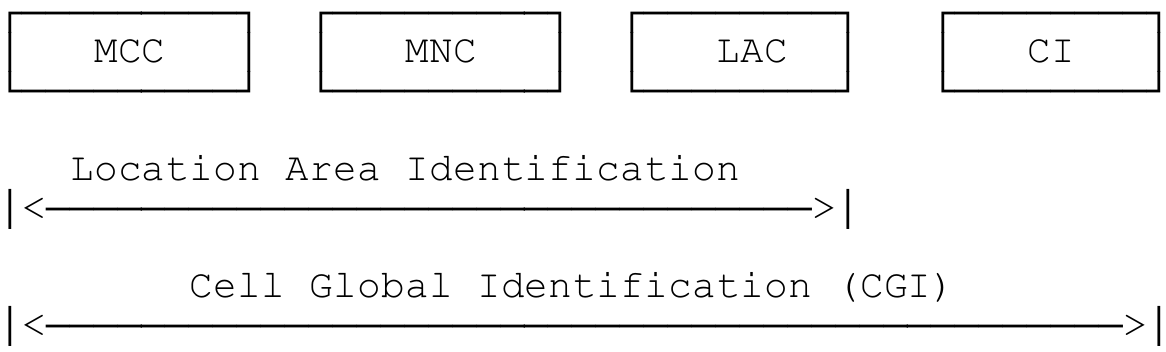
\includegraphics[width=0.7\textwidth]{structure_of_cgi.png}
        \caption{Structure of Cell Global
        Identification~\cite[p.~14]{3gpp_ts_2003}}
        \label{fig:structure_of_cgi}
      \end{figure}


    \section{Mobile Station}

      Finally, the last element of the \gls{plmn} infrastructure is the
      \gls{ms} or \gls{ue}. It consists of the physical equipment used
      by a \gls{plmn} subscriber and is shown on the left of
      \fref{fig:network_architecture}. It comprises the \gls{me} and the
      \gls{sim}. The \gls{me} is the mobile phone itself and contains
      the \gls{imei}, a unique number identifying the equipment, while
      the \gls{sim} is a removable module containing the \gls{imsi}, a
      unique number identifying a subscriber. Like the \gls{auc}, the
      \gls{sim} also stores the subscriber authentication key Ki, can
      execute the A3 algorithm for authentication, and the A8 algorithm
      to generate a session key Kc. The A5 algorithm is executed on the
      \gls{me} to encrypt the communications on the Um interface.
      Finally, the \gls{sim} also stores temporary network data, like
      the
      \gls{tmsi}~\cite{etsi_gsm_2000,etsi_gsm_2001,3gpp_ts_2014-1,3gpp_ts_2015}.
